% This example An LaTeX document showing how to use the l3proj class to
% write your report. Use pdflatex and bibtex to process the file, creating
% a PDF file as output (there is no need to use dvips when using pdflatex).

% Modified

\documentclass{l3proj}
% Below two lines are only to be used if necessary. They shrink the spacing between
% 	list items and save almsot a page worth of space in the document.
% \usepackage{enumitem}
% \setlist[itemize]{noitemsep}
\graphicspath{ {images/} }

\begin{document}

\title{Building Healthy Communities Database}

\author{
Christopher Sean Harris, Documentation, 2128878h \\
David Andrew Brown, Lead Developer, Docker Magician 2137184b \\
David Robertson, Lead Developer, 2135967r \\
Jaklin Yordanova, Documentation and Front End Developer, 2122832y \\
Kiril Ivov Mihaylov, Front End Developer, 2062132m \\
Maria Papadopoulou, Documentation and Front End Developer, 2136603p}

\date{\today}

\maketitle

\begin{abstract}

Building Healthy Communities in Dumfries and Galloway is a community development programme which aims to advance the health and well-being of all individuals within its area, but particularly those in difficult circumstances. Its main goal is to improve the lives of people who may otherwise become isolated, by encouraging participation in initiatives which help keep them physically and mentally healthy, while also promoting the creation and sustaining of social bonds. The programme consists of three different types of participants; \textit{Administrators}, \textit{Volunteers} and \textit{Service Users.} Both \textit{Service Users} and \textit{Volunteers} attend the initiatives that come under the scheme. The difference being \textit{Volunteers} have the added responsibility of running the weekly meetings and recording attendance of \textit{Service Users.} Currently, many of the administrative tasks associated with the scheme are done by hand. Administrators must manually input the data given to them into \textit{\textit{Microsoft} Access}, which is a slow and laborious process.

\end{abstract}

%% Comment out this line if you do not wish to give consent for your
%% work to be distributed in electronic format.
\educationalconsent
%==============================================================================
\section{Introduction}

Third year undergraduates on the Computing Science course of the University of Glasgow undergo a year long team project, the aim of which is to give students the experience of working in a team on an extended software engineering project. The lesson the course instills in students is how to liaise with customers, and use agile software development practices and methodologies to turn this communication into an end product. Another takeaway from the course is the \textit{art} of Retrospection; the act of looking back to see what can be improved in future. With this case study; our intention is to analyse and explore the methodologies we employed in order to better understand their intricacies and how they should be used in a project.

This paper presents a case study of the building of a database system for the public health program 'Building Healthy Communities', and the development practices we used in the process. The \textit{BHC} system is designed to replace the cumbersome, manual database currently in use by the \textit{NHS} team that administers the \textit{BHC} initiatives. It is intended to be a streamlined service, allowing for faster input and retrieval of data. Which before required the cumbersome use of \textit{Microsoft access.} \textit{Service Users} and \textit{Volunteers} will be able to log in and perform tasks that would otherwise require the time of an \textit{Administrator.}

Throughout this study, a more in-depth explanation will be given on how the end product was designed and created. Using not only knowledge gained in our spare time, but also that which has been imparted upon us by courses at the University. More specifically; \textit{Professional Software Development and SIT}, \textit{Interactive Systems 3} and \textit{Database Systems.} The aforementioned courses played a critical role in the development of the end product. By following principles taught to us, it led to the smooth development of the end of product. Which is of a standard and quality that we can all be proud of.
%==============================================================================
\section{Case Study Background}

\subsection{Customer Organisation and Background}
\label{customer}

\textit{Building Healthy Communities} is a programme based in Dumfries and Galloway which consists of a regional partnership of strategic and local representation to help shape and direct, alongside four local area partnerships operating across the region. These area partnerships co-ordinate and take collective action by creating initiatives to tackle community health issues and the root causes of ill health.

The primary method by which \textit{Building Healthy Communities} tackles its main objective is the creation and running of health initiatives. These are regular events, run by community members, for community members, with the aim of bettering the health of individuals and the community as a whole. They foster a sense of well-being, and focus on people who might not otherwise be engaged in social events and feel isolated. Individuals are given the opportunity to become community health volunteers through training and one-to-one support. This allows local citizens to feel active and helpful in their community.

While initiative events are run by volunteers from local communities, the programme itself is run and maintained by a group of \textit{NHS} employed administrators. During the development of the project we had monthly meetings with the administrators. Our interactions with them were instrumental in the shaping of our product, providing requirements and feedback. There was also some incidental contact with another \textit{NHS} employee from the same area running a different project, whose technical advice was of particular use when designing the database and deciding which information needed to be included.

\subsection{Initial Objectives for the Project}
\label{sec:initial-objectives}

The initial objectives for the project were to develop a software which will be used by the service users, volunteers and administrators of the programme. Different types of user have different levels of access to the website. The service users can use the software to complete a small questionnaire and give a regular feedback for the initiatives they attend. Volunteers are an extension to a service user in that they would be able to leave feedback, but also take attendance for the initiatives they are assigned to. Administrators have the access and rights to do everything. They can manipulate data in the database, and view all information that is collected. Like user feedbacks and attendance statistics. Through customer meetings the requirements were changing and adapting frequently, as explained later in the dissertation.

%==============================================================================
\section{Agile Programming, Technologies, and Team Organisation}

\subsection{Team organisation}
\label{sec:organisation}

During the initial team meetings, every team member identified their strong and weak points in order to divide the work. As the website and supporting database needed to be built from scratch, the work required was extensive. Throughout development, everybody contributed what they could. Inevitably, certain team members had a higher level of expertise and thus were tasked with the more complex areas of development. The team discussed various means of communication and decided to avoid the usage of common social media sites. The group-chat application 'Slack' was used throughout the course, which provides a more organised and professional chat room with different channels.

\subsection{Agile Methods}
\label{sec:agile}

Agile methodologies were followed throughout the entire process where sensible. Specifically, they are suitable for small teams and they involve frequent customer meetings because the requirements cannot be fully collected at the beginning of the software development cycle. The project focused around an agile method called "Extreme programming". One of the most useful features that Extreme Programming offers is called 'pair programming.' As the project was developed by students, a lack of experience was a major bottleneck for some aspects of development. Pair programming negates this issue to some extent by allowing team members with different levels of expertise to combine their knowledge and come to the best decision. Additionally, pair programming increases work productivity since working in pairs motivates even the less productive members of the team to contribute. Furthermore, user stories and prototyping played a critical role in understanding the application requirements. Finally, another important feature of Extreme Programming is the automated testing which will be described in more depth in section \ref{sec:backend}.

\subsection{Technologies Used}
\label{sec:tech}

The University Moodle page suggested a litany of technologies  to use for handling the project such as "Ant and Ivy", "Jenkins", "Apache", etc. After a small group meeting and a discussion with the supervisors about what technologies were permitted, the decision was taken to ignore all of the suggestions and use \textit{GitLab} \cite{Gitlab} for our project and repository management.

\textit{GitLab} is a complete repository management system. It not only provided us with a \textit{git} based repository; but also gave us an integrated wiki in which to store documentation, a comprehensive issue tracking system like \textit{Trac}, and a \textit{Continuous Integration} suite in the same vein as \textit{Jenkins}. The combination of all of these features in one discrete package made \textit{GitLab} the obvious choice for us, negating the need for multiple cumbersome systems that we would need to keep track of separately. The next few paragraphs illustrate the reasons why the use of \textit{GitLab} turned out to be a wise choice.

The first major feature \textit{GitLab} provides is the \textit{git} based repository that gives it its name. This repository allowed the team to simultaneously work on the project in different branches, either collaborating on a single section or working individually. With the added benefit of wrapping all of \textit{git's} powerful features into a sleek interface.

The issue tracking system in \textit{GitLab} allowed us to create detailed issues containing checkboxes of tasks, time estimates, comments and more. These issues can be assigned labels; the labels allowed us to see at a glance which area of the project the issue was for (a new feature, documentation, testing etc). Issues were assigned to individual team members, so that those members had a clear focus. \textit{GitLab}'s repository and issue tracking system are linked, which meant that we could create a new branch for each issue easily. This greatly simplified the process of implementing and testing features, by making each small feature its own issue and spawning a branch from it. The feature could then be worked on in isolation, and when complete and tested a merge request could bring those changes back into the master branch. The lead developers would review the code before accepting the request, and either leave a comment about any problems and wait for their resolution, or accept the request, which automatically closes the relevant issue and deletes the merged branch.

\textit{GitLab} also features a \textit{Continuous Integration} suite \cite{ci}, an extremely powerful toolkit that we used to continually test the system upon every commit. We created and continually updated a set of tests that would run on every commit by default, in the hopes of ensuring that no bugs would effect the master branch. The method we used to implement \textit{CI}, was through \textit{Docker}. Which is explained in its own section.

The final useful feature provided by \textit{GitLab} is the wiki. This is an easily editable collection of pages used for the project documents. We created an organised system for documentation, with a sectioned wiki homepage linking to a variety of documentation types, from our design documents, to customer requirements and meetings, to our retrospectives. This simple structure allowed us to keep a very clean and easy to understand collection of documents that could be referred to later, helping us to keep focused and organised.

A decision was now to be made on which technologies were to be used to implement the application itself. Namely, a web application framework was to be chosen. All members of the team had some degree of experience in Django \cite{Django}; however, other alternatives were explored to ensure the best option was selected for this particular project. \textit{Ruby} on \textit{Rails} was a prevailing suggestion, and whilst being conceptually similar to Django, has been around for much longer. \textit{Rails} has a mature and reliable code base, abundant documentation and excellent built in testing support, as seen in section \ref{sec:testing} \cite{Rails}, \cite{DjangoVsRails}. Also, with \textit{Rails} being an industry standard for modern web application development, the team felt it was a valuable experience to develop a large scale application using this framework. With all this in mind, the team chose to go ahead with \textit{Ruby} on \textit{Rails}. One downside of \textit{Rails} is the lack of official programming style reference, something that Django does have. Despite this, many community driven style guides do exist for both \textit{Ruby} \cite{rubyStyle} and \textit{Rails} \cite{railsStyle}. There was high emphasis placed on trying to ensure our code conformed to these style guides. Following a style guide not only helps keep code efficient, but it allows other developers to quickly identify the intent of code because, in theory, everyone should be working to the same style. It also ensures that for projects with multiple developers working simultaneously, a consistent layout is maintained.

\subsection{Retrospective}
\label{retrospective}

In order to regularly summarise the team's progress, the usage of retrospectives was a useful tool. Retrospectives for us was team effort to identify how we were progressing as a team. The creation of retrospectives was done on \textit{Trello}. The criteria used for the retrospectives were the 4L's: Liked, Lacked, Learned and Longed for. A new retrospective was created every time a customer meeting was performed, which indicated the end of a milestone and an iteration. The retrospective process took approximately one hour, allowing every team member to individually outline their thoughts and suggestions about the previous iteration. Following this process, an hour long team meeting took place which discussed the major issues that were outlined and identified through \textit{Trello}. A summary of which was added to our wiki. This process proved to be a highly efficient method of discovering and resolving issues in the team.

\subsection{Team Roles}
\label{sec:roles}

Due to the fact that the team was composed of novice programmers, the team roles were not clearly defined in the beginning. After the first iteration, and we had all identified our strengths, the roles assigned to team members evolved naturally. These roles can be referenced at the beginning of the document. The team voted to elect a leader, The team leader conducted all retrospective meetings and any presentation of the application to the customers. The team leader did not make final decisions alone, apart from where necessary. All team members were of course given the chance to voice their opinions. The team leader's main priority was to organise and delegate tasks to the rest of the team. The team voted fairly to elect David Brown as the team leader since he is one of the lead developers and was by far the most proficient at communicating with the customers. Over time we found that certain team members would face greater difficulties in resolving code-based issues than others, this is why we decided to introduce the concept of 'lead developers'. Since the workload of back end development is substantial, it allowed minor issues to be assigned to other team members, allowing the lead developers to focus on more technical issues.

%==============================================================================
\section{Documentation}
\label{documentation}

After some initial consideration, we decided that fortnightly sprints would be ideal. Each sprint corresponded to the conclusion of a milestone. Issues would then be created, most of which having a deadline of the upcoming milestone. The following portion of the case study will chronologically outline the development process from the requirements elicitation, to the final software presentation.

\subsection{Requirements Gathering}
\label{requirements}

During the first customer meeting, some basic requirements were outlined. Notes were taken during the meeting and a wiki page was created containing a summary of the meeting. Our aim during this meeting was to get a basic understanding of the functional and non-functional requirements for what the website could be. Using our summary and further conversations with the client through email, we managed to establish a solid basis from which to launch the project.

The functional requirements were:
\begin{itemize}
\item An administrator should be able to view all information stored in the database.
\item An administrator should be able to add/remove/modify users and groups that are stored in the database.
\item An administrator should be able to search and sort on specific fields belonging tables.
\item An administrator should be able to view metrics on how particular initiatives are progressing.
\item Different groups of users should have differing levels of permission to the data they can access.
\item Volunteers should be able to view some data about the specific initiatives they are enrolled for.
\item Volunteers should be able to record attendance for initiatives.
\item Provide a facility to gather feedback from service users and volunteers.
\end{itemize}

The non-functional requirements were:
\begin{itemize}
\item The system should be secure.
\item The system has to conform to the Data Protection Act.
\item The system should be stable whilst in use and have a high up time.
\item The system should be able to operate for long periods of time without intervention from system admins.
\item The system should be simple to use.
\item The system should be modular and hence maintainable.
\item The system should be lightweight.
\item The site should be compatible with many web browsers on a range of devices.

\end{itemize}

\subsection{User Stories}
\label{user_stories}

User stories \cite{UserStories} play a critical role in the agile methodologies which we followed. A user story formally describes the state of the application and the basic functionality that a potential user can expect it to have. We compiled a list of Functional and Non-Functional user stories. These helped us tremendously in figuring out not only the flow of the interface, but what features the website could/should have.

These are a few highly representative functional user stories:
\begin{itemize}
\item As an administrator, I want to add a member to the database, so that they can join a group.

	\begin{enumerate}
	\item Add an activity to add a person
	\item Add an activity to enter their information
	\item Add an activity for choosing groups
	\item Create a query for retrieving groups
	\end{enumerate}

\item As a volunteer, I want to be able to register attendance at my group(s), so that I can contribute data.

	\begin{enumerate}
	\item Create a query to retrieve groups I run
	\item Add an activity to log attendance
	\item Create a query for members of the group
	\item Add an activity to enter attendance per member
	\end{enumerate}

\item As a member, I want to be able to log in, so that I can view my information.

	\begin{enumerate}
	\item Add an activity to log in
	\item Add an activity to enter log in information
	\end{enumerate}
\end{itemize}

Some non-functional user stories are:

\begin{itemize}
\item  As an administrator, I want to replace a member's name with numbers in the database, so that I can find them easier.

	\begin{enumerate}
	\item Create a query for retrieving a person
	\item Add an activity to update a person's information
	\item Create a warning message for wrong type of input
	\item Do not allow this modifications to be saved
	\end{enumerate}

\item As a volunteer, I want to be able to have access to the database, so that I can add a new program that the administrators haven't added yet.

	\begin{enumerate}
	\item Restrict the "Add a new page", "Add a new page", "Add a new member", etc buttons to can be only accessed from administrators
	\end{enumerate}

\item As a member, I want to be able to add or delete a group that I am part to, so that I can register my self to new groups or delete me from the old ones.

	\begin{enumerate}
	\item Restrict the member's redirected page to do very basic tasks
	\item Do not provide this functionality to members.
	\end{enumerate}
\end{itemize}

\subsection{User Scenarios}
\label{user_scenarios}

Although user stories provide a clear outline of the features and attributes the system should have; Scenarios helped us to concretise how our 'real world' users could would interact with the system.
Example scenarios:
\begin{itemize}
\item Carolyn is an administrator in the \textit{Building Healthy Communities} program. She is in charge of tracking the volunteers progress and checking if they are doing their work correctly. It is important for the program to not only track the attendance of service users and their feedback but also to track the same for volunteers. This is vital for ensuring the programme is being run correctly and also would be an advantage in building the relationship between service users and volunteers.

\item Rebecca is a volunteer in the \textit{Building Healthy Communities} program at the Arts group. She is currently working with a group of eight people. At the end of every session she collects attendance. The process of submitting attendance on paper is very time consuming. She would prefer to have a website to input this data, to save her time and to provide administrators with instant access to the information.

\end{itemize}

\subsection{Wireframes}
\label{wireframes}

After creating and compiling the previously mentioned documentation, the next process was to develop wireframes. Wireframes were the final goal of the first milestone and the only requirement specified by the customers for the next meeting. After researching wireframe and prototyping tools, \textit{Balsamiq} proved to be the most suitable application for our needs. \textit{Balsamiq} is a very useful application, easy to use and focuses on the creation of wireframes. Before we started sketching in \textit{Balsamiq}, we decided to take an initial low-fidelity route and sketch the wireframes on paper. Low-fidelity wireframes are often a good starting point as they are quick to produce and thus many designs can be produced rapidly, allowing the best from a selection to be chosen to move ahead with.

A wireframe of the login page which was presented to the customers can be found in \autoref{fig:initialWireframe}.

\begin{figure}[ht]
\centerline{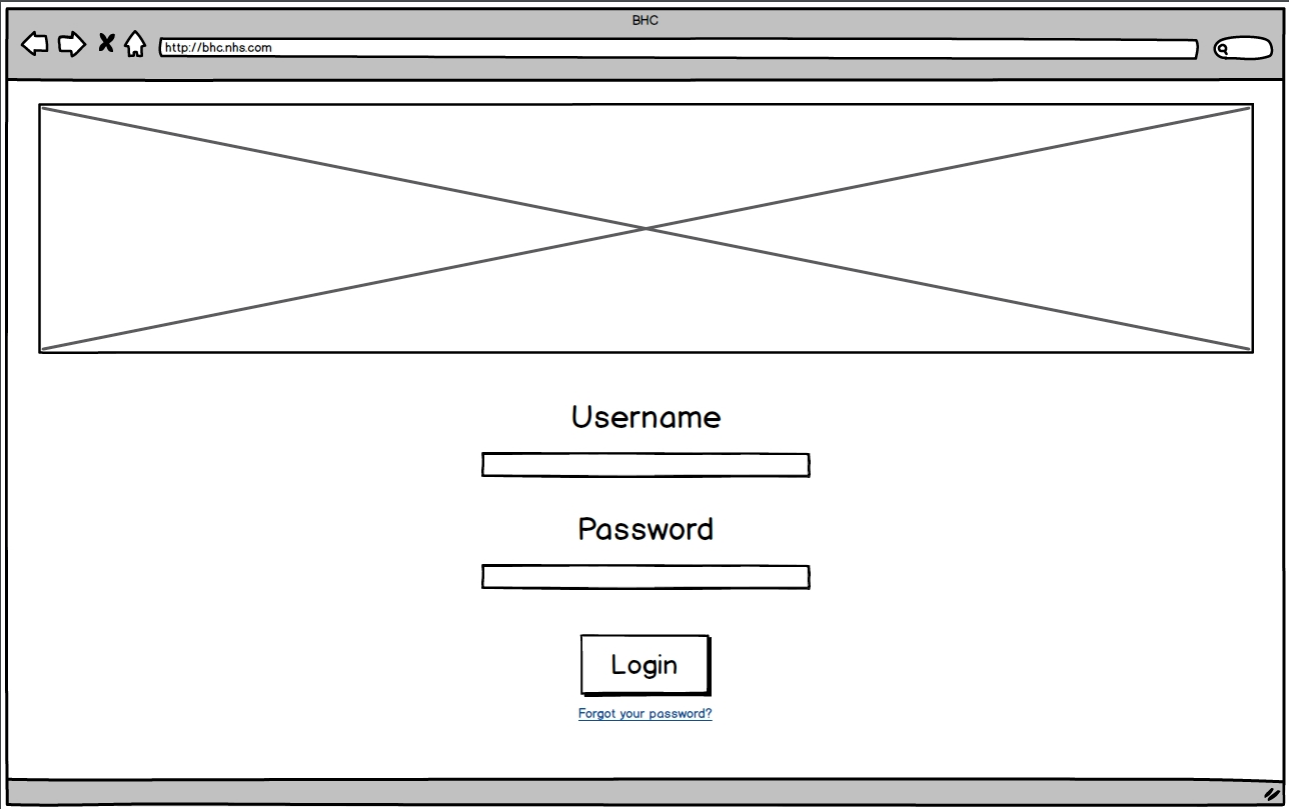
\includegraphics[width=\textwidth, height=\textheight, keepaspectratio]{wireframe.png}}
\caption{Wireframe of the login page}
\label{fig:initialWireframe}
\end{figure}

\subsection{End of First Milestone}
\label{sec:milestone1}

The second customer meeting was held on the 16th November. In the meeting some example user scenarios were showed to the customer and a brief demo was given through our interactive wireframes. The customers expressed their opinion about our current progress and what they expect to be completed by the next customer meeting. After the meeting, the team completed a retrospective. We found that during the interim period between this meeting and the last, we as a team improved our knowledge on using \textit{GitLab} as a project management tool. The biggest issue we identified was that further and more frequent communication with the customers was needed. As some aspects of the application were left ambiguous and misunderstood. Not entirely our fault, but just teething problems that arose as the customers fine tuned their ultimate vision of the project/website.

%==============================================================================
\section{Design of the Website}
\label{sec:design}

\subsection{Objectives}
\label{sec:design-objectives}

For the next iteration, we outlined our main priorities and assigned issues to everyone. The design of the ER diagram was one of our top priories, but by this point the process of implementing the application was well underway.

\subsection{ER Diagram}
\label{sec:er}

An Entity-Relationship diagram \cite{er} is a useful tool for clarifying the development of every database supported application. Having an ER diagram represents clearly the relationships between entities and the attributes that belong to them. Having a diagram to work from meant that development went smoother than expected. Using \textit{Rails's} powerful ActiveRecord system allowed us to quickly design and implement the database. The full ER diagram is shown in \autoref{fig:er}.

\begin{figure}
\centerline{\includegraphics[width=\textwidth, height=\textheight, keepaspectratio]{er2.png}}
\caption{Entity Relationship Diagram}
\label{fig:er}
\end{figure}

\subsection{Component Architecture}
\label{sec:component}

\textit{Ruby on Rails} uses a model-view-controller architecture pattern, which allows our team to develop an agile application. The model layer represents the logic of the application and the management of interactions with elements in the database. The view is the front-end of the application and the HTML files with embedded \textit{Ruby}. Controllers interact with models and views responding to requests from a user. Which in turn generates the pages that a user will see. Additionally in this diagram, you can see our use of Docker. This is further explained in \autoref{sec:docker}.

\autoref{fig:ca} demonstrates visually the component architecture of our application.

\begin{figure}[ht]
\centerline{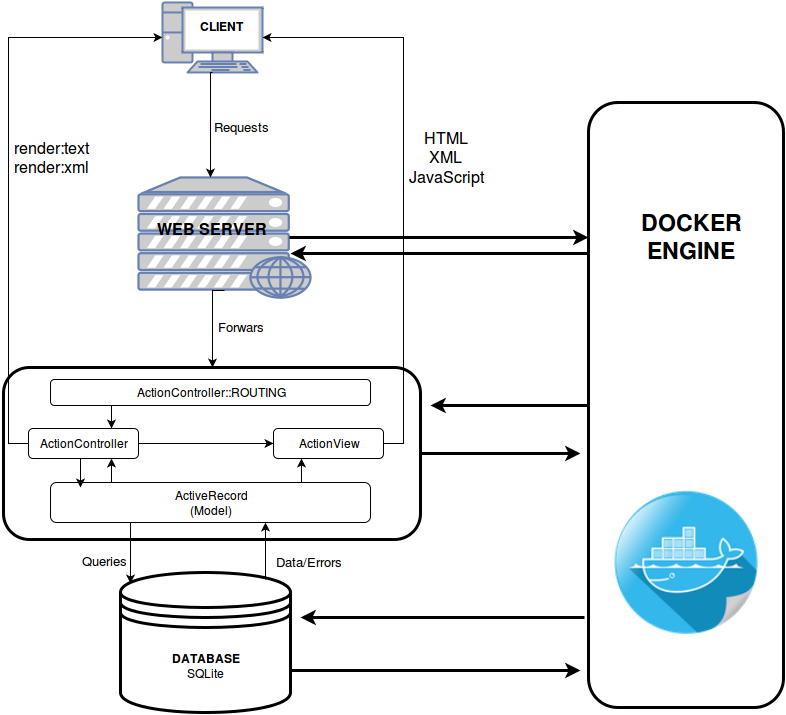
\includegraphics[width=\textwidth, height=\textheight, keepaspectratio]{component.png}}
\caption{Component Architecture}
\label{fig:ca}
\end{figure}

\subsection{Initial Prototype}
\label{sec:prototype1}

Having the basic database structure, initial prototypes of the page were created, in order to discuss potential design changes. The first version of the page can be found in \autoref{fig:oldhome}.

\begin{figure}[ht]
\centerline{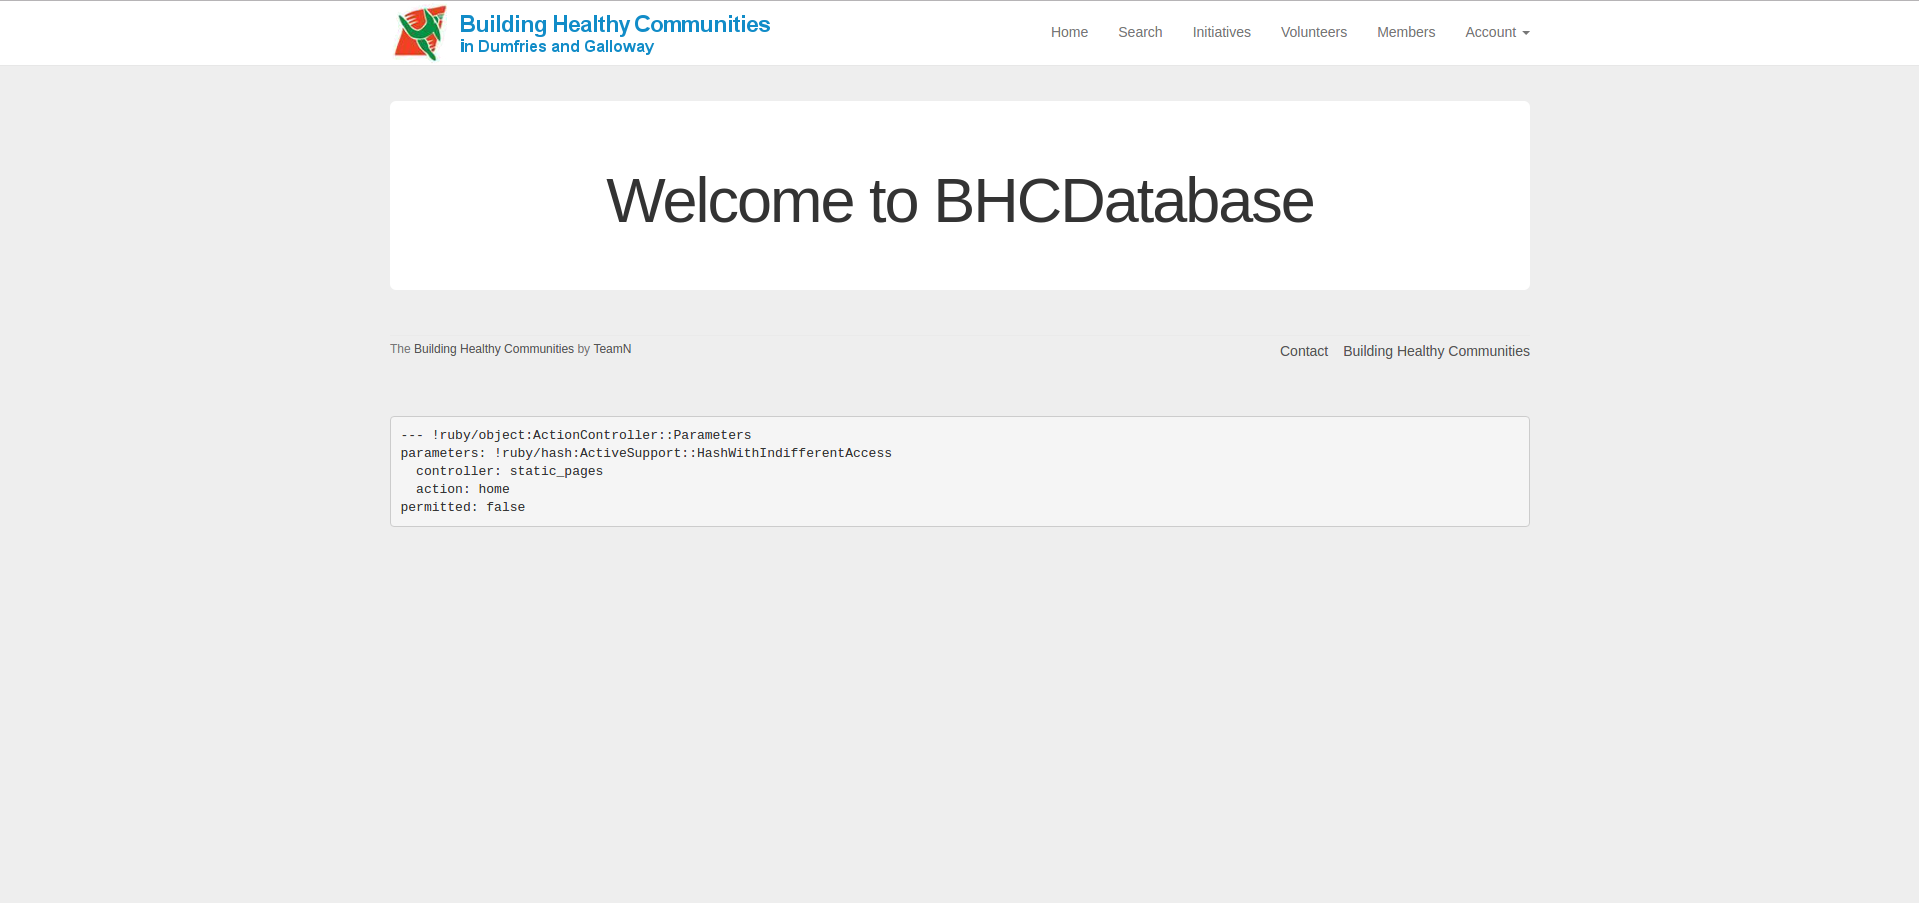
\includegraphics[width=\textwidth, height=\textheight, keepaspectratio]{oldhome.png}}
\caption{Initial Prototype}
\label{fig:oldhome}
\end{figure}

The design of the website originally was basic, not very colourful. This was intentional, to help bring a modern and simplistic style to the website. However when we showed this to the customer, they didn't really like this approach. They requested that more colour was injected into the website, following the colours of the \textit{BHC} scheme. This change resulted in the look and feel of the website that we continued through the entire development of the website.

\subsection{Final Prototype}
\label{sec:prototype2}

The second design was more simplified in terms of account organisation. The customers clarified one of their requirements regarding that the service users would not be able to sign up on their own, which had the consequence of deleting this feature as it was already fully implemented. This new prototype/design can be found in \autoref{fig:newhome}. Note that this is not the final design of the website but the final prototype that we presented to the customers early on in development.


\begin{figure}[ht]
\centerline{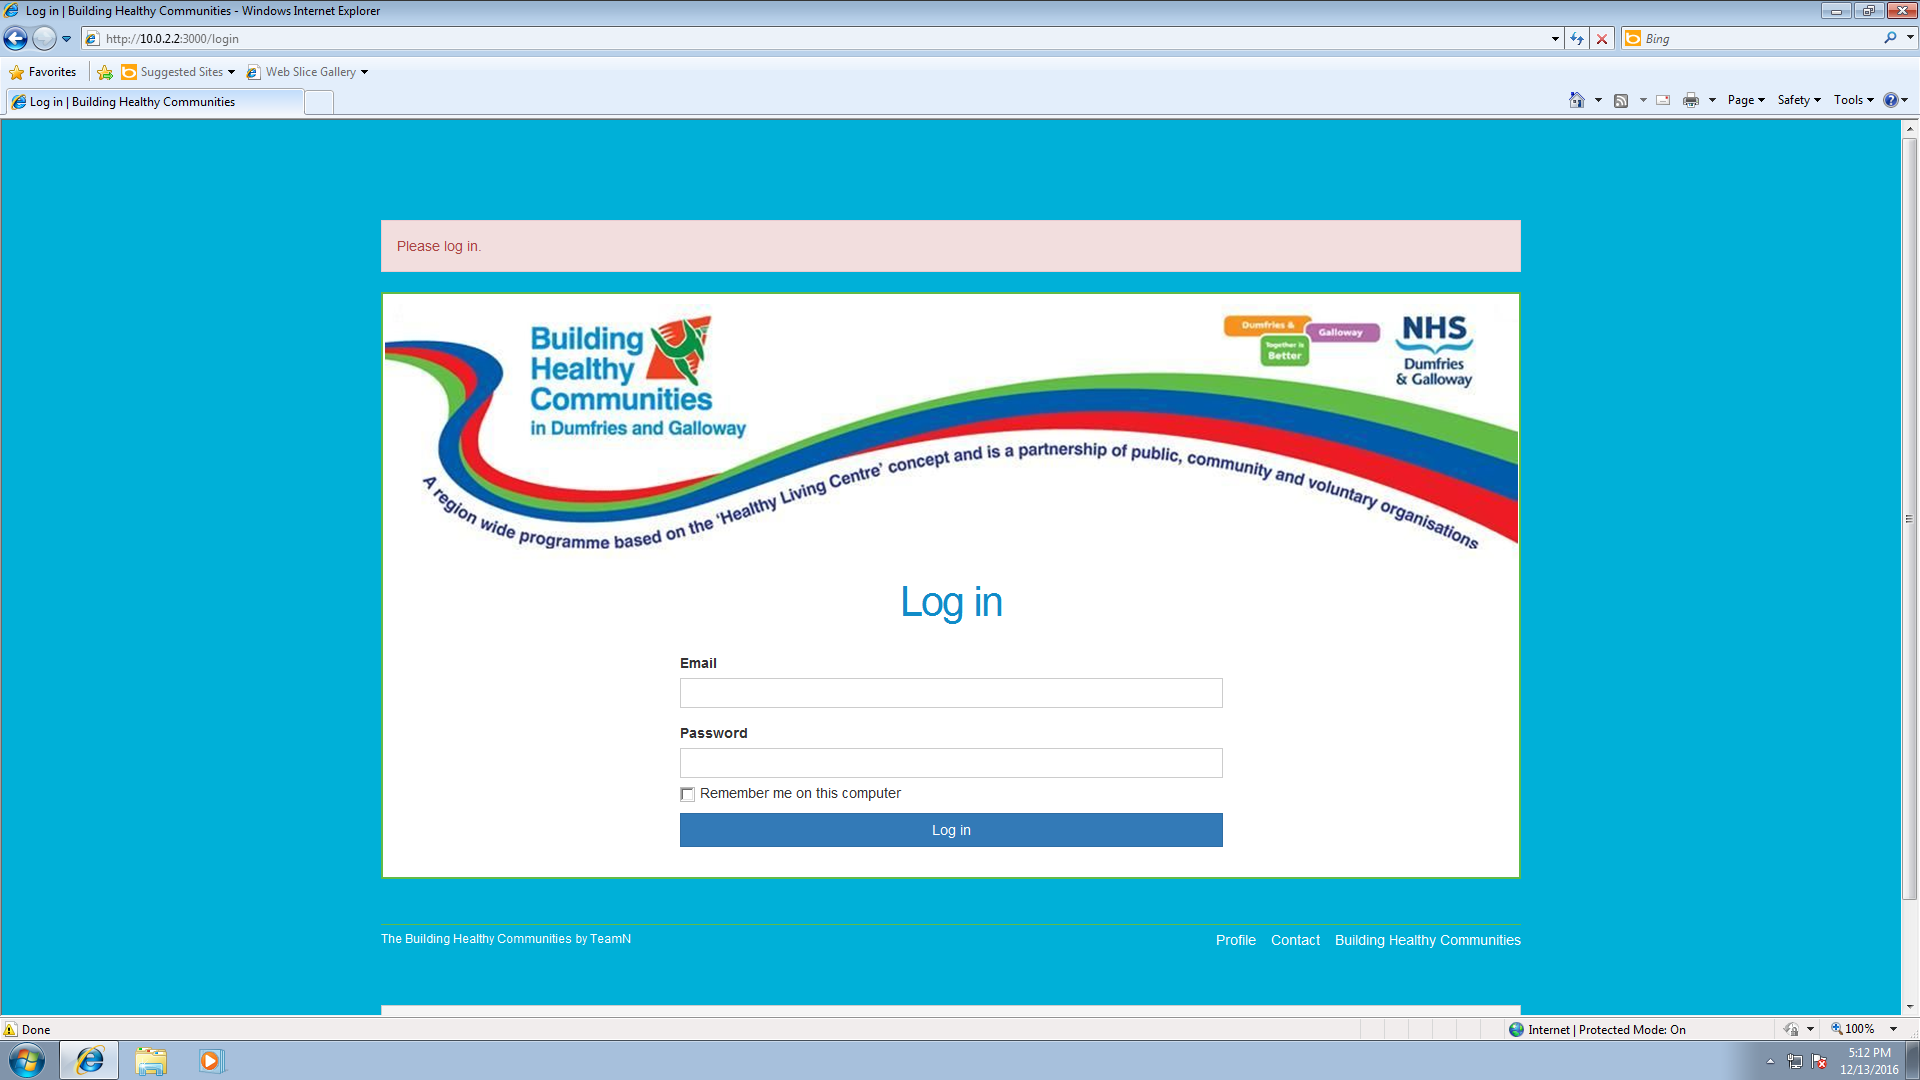
\includegraphics[width=\textwidth, height=\textheight, keepaspectratio]{newhome.png}}
\caption{Second version of the prototype}
\label{fig:newhome}
\end{figure}

\subsection{End of second and third milestone}
\label{sec:milestone23}

The above section generally outlines the progress in the second and third milestone. The progress we made was steady. By the 7th of December, a third customer meeting was held which was mainly used for further clarifications about the software implementation and navigation through the early version of the website. Once we were able to walk the customers through a functioning version of the website, it proved to be an invaluable part of the meetings. They were quick to point out flaws, and it allowed everyone to see how things could be improved. Additionally, they requested a new feature which hadn't been identified to us perviously, the ability to 'fund' entities. A funder could fund the progress of a particular initiative, user or medical addition. This feature addition was a costly addition, but once it was added to the ER diagram the solution to how to implement it became clear.

The retrospective performed by the end of the third milestone, showed some lack of communication. The team did not consider this a major issue since there was in theory a three week holiday during this time period. Although some members of the team continued work over Christmas, and this is when our \textit{CI} system and deployment strategy was implemented. Additionally, the team lacked clarification on some basic features of the website with the customers. All the issues outlined in the second retrospective, were solved during the next. The team was more organised and communicative. Upon our fourth customer meeting; lack of clarification on features that was raised as an issue in the previous retrospective was now solved. We approached them with a clear list of questions that we had compiled and created an issue for. We continued doing this for the rest of development and it helped us tremendously.

%==============================================================================
\section{Backend Development}
\label{sec:backend}

\subsection{Objectives}
\label{sec:backend-objectives}

Before the fourth milestone, the next objectives were outlined. By this point in development a feature rich version of the website was expected to be delivered, the main goals were to resolve opened issues that were raised from the previous retrospective and customer meeting. The most critical issues that were raised were the newest demands that the customers had, most notably the 'funder' feature outlined above.

\subsection{User Authentication}
\label{sec:authentication}

One of the most important features of the website is the protection of user information. 'User authentication' \cite{authentication} is the process in which user credentials are compared with the information that is kept in the database. Improper development of user authentication could lead to the leak of personal information from one user to another, or the ability for every user to edit the database in any manner they wish. We researched the best practices of developing a highly secure means of user authentication. A popular \textit{gem} for user authentication is "Devise" \cite{devise}. Some of its features are the ability of assigning multiple models in at the same time and its modulation. Although \textit{Devise} is an excellent tool. The features it provided were unnecessarily bloated and would slow down the development of the website. The user authentication model we decided upon is based outlined in a book called "Ruby on Rails Tutorial (Rails 5)" written by Michael Hartl \cite{railsTut}. The book provides tutorials on how to construct your own method of user authentication, using another \textit{gem} called \textit{bcrypt} allowed us to store a cryptographically secure password in our database.

\subsection{Browser and Mobile Compatibility}
\label{sec:compatibility}

The scope for browser compatibility was quite broad. Throughout the customers' meetings it was clear that broad support of the most popular browsers is essential and that the website should function on both \textit{iOS} and \textit{Android} (Running in both tablet and mobile form).
An issue that was raised very early, was the support of \textit{Internet Explorer} version 7 and above. The earliest \textit{Internet Explorer} version we chose to eventually support is \textit{IE 8}. This is because IE8 comes as standard with \textit{Windows 7} which still is supported by \textit{Microsoft}. Although possible, we have chosen not to support \textit{IE 7} due to it coming with \textit{Windows Vista} which has 'Extended support [only] until 11 April 2017.' The final decision not to support \textit{IE 7} was more from a security standpoint than technical feasibility. When we discussed this with the clients they were satisfied. Mobile browser compatibility was one of our major points of focus. The experience we focused on most was that of a volunteer. A volunteer being able to take attendance from their phone was very important for us, so this experience was prioritised above all others to work perfectly on mobile. A screen shot shows how the website looks on mobile \autoref{fig:compatibility}.

\begin{figure}[ht]
\centerline{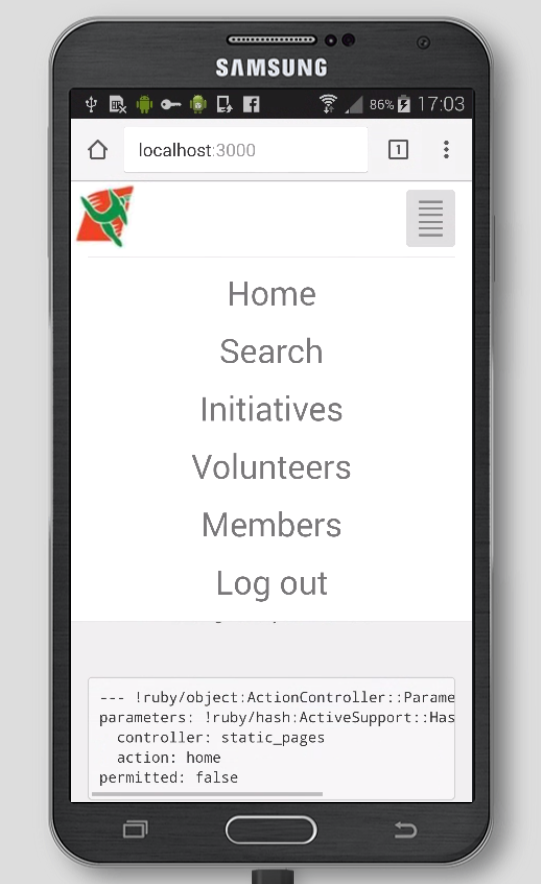
\includegraphics[ scale=0.3]{mobilePrototype.png}}
\caption{Mobile Compatibility Prototype}
\label{fig:compatibility}
\end{figure}

\subsection{Testing}
\label{sec:testing}

An integral step in developing an application is constructing a test suite that is as complete and robust as possible. It is vital that testing begin early in project development, as the costs required to implement defect tests late in the process can be extremely costly. With this is mind, testing began almost immediately, any time a feature was to be implemented, the corresponding tests were to be written before the issue could be closed. The tests were constructed using Rail's built-in testing framework. Upon creation of an app in \textit{Rails}, a 'test' directory is created which holds many other directories intended to contain different testing groups. For example, the 'controllers' directory holds all tests for the controllers and the 'integration' directory holds all tests that involve many controllers interacting together. When creating a model or a controller, the skeleton code for the tests is automatically generated and placed within the corresponding directory. 'Fixtures' are a way of creating and organising test data. On top of using Rail's testing, the \textit{SimpleCov} \textit{gem} was introduced. \textit{SimpleCov} is a code coverage analysis tool which amongst many other things, displays coverage statistics upon test execution. It also generates a 'coverage' folder which contains interactive documentation displaying the code coverage of each file, which lines were hit, and how many times. The application's tests were designed in an attempt to ensure correct functionality in as many target areas as possible, this includes: controller execution, model validations, uniqueness validations, page restriction validations, etc. Tests were not designed to achieve a high test coverage. Whilst lines covered does give a good indication of which areas of the project need attention, it should not be used as a defining mark for 'good' test coverage. It is perfectly possible to have extremely high test coverage, with relatively meaningless, superficial tests.

% --------------------------------------------------- %

\subsection{Docker}
\label{sec:docker}

\textit{Docker} is a very modern way to package, deploy, and build applications. It works on the principle of \textit{images}, that contain your code and the supporting libraries for them. A way we liked to think of it was like \textit{virtualenv} for entire operating systems. Not entirely accurate but it helped us as a team come to grips with \textit{Docker}. It allowed us to build our application in away that meant it was truly portable. More importantly, truly deployable.

The choice to use \textit{Docker} for both testing and deployment wasn't so much a conscious decision as it was one of professionalism. When we started to explore \textit{Continuous Integration} through \textit{GitLab}, it became clear that \textit{Docker} was one of the best means of doing this. There were easier paths we could follow, but to deliver the best product we could meant using \textit{Docker}. Implementing this became one of the hardest challenges of the entire project. None of us had used \textit{Docker} before and to go from not knowing what it was, to having our full deployment and testing suite built on \textit{Docker} was very satisfying. In \textit{GitLab}, every project implementing \textit{CI} has a \textit{gitlab-ci.yml} file. That file is customised per project, to inform \textit{GitLab's} runners how to build the project and what to do. For testing, we have one \textit{Dockerfile} that contains the instructions for how to build an image of our program designed solely for testing. The notable difference between this image and the production setup, is that we use \textit{SQLite} in the same image as \textit{Rails} for testing. \textit{GitLab} spawns a container from this image and runs our test suite, all automatically. This happens on every commit and on every branch. This allowed us to know, at all stages in development, on a commit by commit basis what tests were passing. The next, and more challenging step was to build and deploy the website from the \textit{CI} suite.

Only on master, with every commit, \textit{gitlab-ci.yml} instructs \textit{GitLab} to use a \textit{Docker Compose} file to build our production website. Which is a means of using several \textit{Dockerfiles} together at the same time. Think of it like scripting the commands required to start the individual containers and link them together. \textit{Docker Compose} uses two other \textit{Dockerfiles} to build custom images for us. One for \textit{Rails} and one for \textit{nginx}. It relies also on the official \textit{PostgreSQL} to build our database image. \textit{GitLab} builds the aforementioned three images, and then spawns containers from them. This meant that on our server, there exists at all times, a functioning and deployed version of the website. This website is supported by three containers. One for our web server \textit{nginx}, one for the \textit{Rails} application itself and then one for \textit{}. Splitting the application across three containers was the single most challenging aspect of the project for those involved. With a lack of reference guides on how to do this, it took many man hours. In the end though, it was worth it. Splitting concerns across containers is the best practice for using \textit{Docker}. Not only giving us great experience for the future, it meant that we were very confident that our application was ready for a stable and scalable deployment at all times.

\subsection{End of fourth milestone}
\label{sec:milestone4}

The fourth milestone was successfully completed with all its major goals achieved. The website was successfully presented to the customers on the customer meeting performed on the 23rd of February. Although some minor features were not yet implemented, a fully working version was delivered and in the following month all the features were progressively added. In February we provided the clients with a working version of the website that we hosted on \textit{Heroku}. We used \textit{Heroku} for this because accessing the \textit{Docker} version that is hosted at the University requires \textit{ssh local forwarding.} A questionnaire was given alongside the link to the website, which is explained in \autoref{sec:app-eval}. The customers made more last minute demands to the team upon using the website. These additions were added to the next milestone.

%==============================================================================
\section{User Documentation}
\label{sec:user_doc}

One of the most essential parts of documentation we wanted to produce was a comprehensive user guide. As this project is built for a University Course, we would no longer be maintaining it afterwards. So it was very important for us to produce an easy to follow and understandable user guide. In the case someone else takes over the project, a clear guide on how to use the website would be present for them to reference. We split the guide into three sections: one for administrators, one for volunteers and one for service users. This allowed us to target our guide, adjusting our wording and language accordingly, to personalise the guide for each audience. We focused on the basic tasks that each category of user would perform, and produced genuinely useful guides for our website.

%==============================================================================
\section{Formative Application Evaluation}
\label{sec:app-eval}

A Formative Application Evaluation is a process in which a developer receives objective feedback, useful comments and suggestions about their product. Sent in combination with one of our early drafts of a user guide \autoref{sec:user_doc}, we gave the clients a short questionnaire to perform after using the website. We focused our questions mainly upon navigation and \textit{understanding} of the website, as many other flaws had been picked up and discussed at the last client meeting. The goal of our questionnaire was to study whether the customers were able to navigate the website, and to what extent they were successful in achieving their goals. We used \textit{Google Forms} to make the questionnaire, and we provided them with questions such as:
\begin{itemize}
 \item In general do you like the look and the feel of the website?
 \item Have you found trouble performing search queries in the website?
 \item Have you faced any difficulties in adding new sessions, users, questions and so on?
\end{itemize}

As a consequence of having only a small number of responses, the results were rather qualitative than quantitative. The clients gave us the really useful feedback in the text fields we gave them. They identified subtle issues that we hadn't considered, and proved to us the value of physically allowing the client to use the our product. By the next customer meeting we were able to show them that most, if not all, of their difficulties and complaints had been resolved.

%==============================================================================

\section{Challenges}
\label{challenges}

Developing a program from scratch, always creates some major challenges. The second and third retrospective were extremely representative in the matter of stating major challenges and proposing possible solutions. A very common issue that was experienced during the software development process was the development of test cases. Tests were one of the most time consuming tasks since every small aspect of our website had to be tested to the best of our abilities. At times this was difficult, as we had other more pressing tasks. By the end of development however, our test cases were very thorough; with 278 individual tests we feel confident we have done our best.

Developing the schema to support the program was one of our biggest challenges. We would frequently follow \textit{red herrings} regarding how to support certain features. From which we would have to back track and delete branches, to explore a different avenue. A useful reference guide for us was our \textit{Database Systems} course. We would attend the lectures and either have \textit{eureka} moment on how to solve a problem we were having. Or we would discover an approach we were taking was fundamentally wrong. This led to the efficient use of our database that we have now.

In every project, clients will constantly change their minds about things, or have ideas for new features. The biggest of which our client hit us with was that of 'Funding.' This was quite late on in development, and would require some major additions to our website. Not only were extensive changes to our database needed, seven more tables to be precise, but many additional pages were needed too. Plus the further revision of our ER diagram. Funding became our top priority, and we managed to integrate this feature quicker than we expected. Owing perhaps to our efficiency and experience of working with \textit{Rails} by this point.

A challenge that the clients asked of us; was that the website, almost feature complete, be delivered to them during February. This increased the pressure on us immensely and changed our development direction. Working up to the February deadline, we had to focus our attention more on testing and \textit{user experience} than on new features. We were able to successfully deliver the website in a fully functional state. By that, we mean that there was \textit{no} possible way to break or crash the website through simple button clicks and navigation. Getting them the website meant not only better feedback from them, but gave us the confidence and motivation that we were on the right track, and building them the product they wanted.

The choice to use \textit{Docker} was one of the biggest challenges that faced us. Over Christmas, some fifty plus man hours were spent in incorporating the use of \textit{Docker} into our project. In the end though, it was worth it. It let us ensure the client that eventual full scale deployment was possible, and allowed us to easily test and build the application. High availability and reliability on our server in the University showed us that our website and supporting back end was robust enough to see real world use.

%------------------------------------------------------------------------------
\section{Final Customer Day}
\label{sec:finalDay}

On the 22nd of March we gave the final demonstration of our product. As a team, we had to present our product to: clients, lecturers and our fellow peers. Bu this point, the website was feature complete and we were able to show the clients exactly what we would be delivering to them. This was quite an achievement, as eight days before the demo, the customers informed us that we needed to change the structure of the feedback/questionnaire that users could complete. We managed to integrate these changes fairly quickly, which allowed us to show the full production version of our website hosted through \textit{Docker} on our server. Which we thought to be quite special, as the website we showed was built and deployed all automatically through our \textit{CI} setup on \textit{GitLab}. We didn't need to specially prepare the demo at all.

The demonstration lasted approximately 20 minutes and was comprised of a short presentation and a live demo of our website. With the demo, we tried to tell a \textit{story.} First we logged in as a service user to show their functionality of leaving feedback, and to put in a request to have some of their details changed. Next we logged in as a volunteer, and showed attendance taking of an initiative. Lastly, we logged in as an administrator. We walked through all of the major features of the website, and showed us handling the request that we had submitted earlier. Through performing the demonstration in this way, we hoped that we could show a real world example of how our website could be used. After the demonstration had finished, the customers expressed their gratitude to us for the work we had done. We were asked questions by a several people, whom appeared to be satisfied by our answers. After the demonstration, the clients asked us to ensure a version was available for them to use for further testing. Which we took as a compliment in that we had at least achieved enough in that they were interested in adopting our product.

%------------------------------------------------------------------------------
\section{Conclusion}

Upon reflection, designing and implementing our project was every bit as challenging as we first thought. Considering the team consisted of six novice students, the resulting website is something we can be very proud of. Having real customers to deal with was a welcome and fun challenge.

Agile programming methodologies proved their usefulness throughout the entire development cycle. Pair programming played a critical role in terms of identifying bugs and errors in the code; allowed us to learn \textit{Rails} and \textit{Ruby} and develop relationships as a team. Communication was vital both within the team and with the customer. Though we faced a few communication issues, we quickly learned to communicate more efficiently.

% Putting in practice so many technologies such as Ruby and Docker was undoubtedly one of the hardest tasks that the team had to undergo. Thus, during the Christmas break a wiki page was created which pointed out many useful resources for self-studying and self-practicing.

The project helped illustrate to us the true importance of test cases. Although an arduous process, testing found very subtle bugs within our program that we wouldn't have otherwise discovered. Bugs that could have compromised the entire project. Through our integration with \textit{GitLab CI}, failing tests couldn't be ignored. We had a very strict system for using \textit{git}. Each issue had its own branch, and we disallowed ourselves to commit directly to master unless it was safe to do so. Merge requests were made for every merge, and we encouraged all team members to look over changes before merges took place. Strict branching rules allowed us to stay \textit{agile} in development, and ensured that at all times the master branch represented a fully working version of our website. How \textit{GitLab} integrates \textit{CI} with branching is most superb, it tells you very visibly if a branch you are trying to merge has failing tests. At all merges we made sure that all tests passed in the respective branch before the merge was allowed.

Delivering a quality end product means nothing if it is not what the client wanted. As last minute changes came in from the client at multiple stages in development, we learned that sometimes we just had to say sorry to the client. Informing them that the feature or request was too large to be implemented at short notice. Of which they were always appreciative of our honesty. The end product features all of the requests they had, so in the long run we only had to disappoint them on a select few, short term, occasions. Promising features that couldn't be delivered on time would result in a mistrustful atmosphere between us and the client. Through being honest we managed to avoid this, and it allowed us to have an \textit{easy} and amicable relationship with the client.

Working with \textit{real} clients has proved to be an invaluable experience. For all of us. It's one thing to receive an \textit{A} from a piece of coursework, but to bring about a smile or a gleeful reaction in our clients was quite special. The project was a big challenge, all of us learned valuable lessons throughout development. That you can't always rely on team members to have the same proficiency in areas as you. That effective leadership is vital for some projects, and that true team work can speed up development tremendously. Lastly, that clients can be fickle, and the best thing to do is work with them honestly and openly. We only hope that our project was of a quality and standard that the \textit{BHC} choose us as their platform. Our project and effort will hopefully bring a tangible difference to their efforts, that ultimately benefits peoples lives. That for us, is rather special.

%==============================================================================

\newpage
\bibliographystyle{plain}
\bibliography{dissertation}

\end{document}
